% Options for packages loaded elsewhere
\PassOptionsToPackage{unicode}{hyperref}
\PassOptionsToPackage{hyphens}{url}
\PassOptionsToPackage{dvipsnames,svgnames,x11names}{xcolor}
%
\documentclass[
  letterpaper,
  DIV=11,
  numbers=noendperiod]{scrartcl}

\usepackage{amsmath,amssymb}
\usepackage{iftex}
\ifPDFTeX
  \usepackage[T1]{fontenc}
  \usepackage[utf8]{inputenc}
  \usepackage{textcomp} % provide euro and other symbols
\else % if luatex or xetex
  \usepackage{unicode-math}
  \defaultfontfeatures{Scale=MatchLowercase}
  \defaultfontfeatures[\rmfamily]{Ligatures=TeX,Scale=1}
\fi
\usepackage{lmodern}
\ifPDFTeX\else  
    % xetex/luatex font selection
\fi
% Use upquote if available, for straight quotes in verbatim environments
\IfFileExists{upquote.sty}{\usepackage{upquote}}{}
\IfFileExists{microtype.sty}{% use microtype if available
  \usepackage[]{microtype}
  \UseMicrotypeSet[protrusion]{basicmath} % disable protrusion for tt fonts
}{}
\makeatletter
\@ifundefined{KOMAClassName}{% if non-KOMA class
  \IfFileExists{parskip.sty}{%
    \usepackage{parskip}
  }{% else
    \setlength{\parindent}{0pt}
    \setlength{\parskip}{6pt plus 2pt minus 1pt}}
}{% if KOMA class
  \KOMAoptions{parskip=half}}
\makeatother
\usepackage{xcolor}
\setlength{\emergencystretch}{3em} % prevent overfull lines
\setcounter{secnumdepth}{-\maxdimen} % remove section numbering
% Make \paragraph and \subparagraph free-standing
\ifx\paragraph\undefined\else
  \let\oldparagraph\paragraph
  \renewcommand{\paragraph}[1]{\oldparagraph{#1}\mbox{}}
\fi
\ifx\subparagraph\undefined\else
  \let\oldsubparagraph\subparagraph
  \renewcommand{\subparagraph}[1]{\oldsubparagraph{#1}\mbox{}}
\fi


\providecommand{\tightlist}{%
  \setlength{\itemsep}{0pt}\setlength{\parskip}{0pt}}\usepackage{longtable,booktabs,array}
\usepackage{calc} % for calculating minipage widths
% Correct order of tables after \paragraph or \subparagraph
\usepackage{etoolbox}
\makeatletter
\patchcmd\longtable{\par}{\if@noskipsec\mbox{}\fi\par}{}{}
\makeatother
% Allow footnotes in longtable head/foot
\IfFileExists{footnotehyper.sty}{\usepackage{footnotehyper}}{\usepackage{footnote}}
\makesavenoteenv{longtable}
\usepackage{graphicx}
\makeatletter
\def\maxwidth{\ifdim\Gin@nat@width>\linewidth\linewidth\else\Gin@nat@width\fi}
\def\maxheight{\ifdim\Gin@nat@height>\textheight\textheight\else\Gin@nat@height\fi}
\makeatother
% Scale images if necessary, so that they will not overflow the page
% margins by default, and it is still possible to overwrite the defaults
% using explicit options in \includegraphics[width, height, ...]{}
\setkeys{Gin}{width=\maxwidth,height=\maxheight,keepaspectratio}
% Set default figure placement to htbp
\makeatletter
\def\fps@figure{htbp}
\makeatother

\usepackage{booktabs}
\usepackage{longtable}
\usepackage{array}
\usepackage{multirow}
\usepackage{wrapfig}
\usepackage{float}
\usepackage{colortbl}
\usepackage{pdflscape}
\usepackage{tabu}
\usepackage{threeparttable}
\usepackage{threeparttablex}
\usepackage[normalem]{ulem}
\usepackage{makecell}
\usepackage{xcolor}
\usepackage{caption}
\KOMAoption{captions}{tableheading}
\makeatletter
\@ifpackageloaded{caption}{}{\usepackage{caption}}
\AtBeginDocument{%
\ifdefined\contentsname
  \renewcommand*\contentsname{Table of contents}
\else
  \newcommand\contentsname{Table of contents}
\fi
\ifdefined\listfigurename
  \renewcommand*\listfigurename{List of Figures}
\else
  \newcommand\listfigurename{List of Figures}
\fi
\ifdefined\listtablename
  \renewcommand*\listtablename{List of Tables}
\else
  \newcommand\listtablename{List of Tables}
\fi
\ifdefined\figurename
  \renewcommand*\figurename{Figure}
\else
  \newcommand\figurename{Figure}
\fi
\ifdefined\tablename
  \renewcommand*\tablename{Table}
\else
  \newcommand\tablename{Table}
\fi
}
\@ifpackageloaded{float}{}{\usepackage{float}}
\floatstyle{ruled}
\@ifundefined{c@chapter}{\newfloat{codelisting}{h}{lop}}{\newfloat{codelisting}{h}{lop}[chapter]}
\floatname{codelisting}{Listing}
\newcommand*\listoflistings{\listof{codelisting}{List of Listings}}
\makeatother
\makeatletter
\makeatother
\makeatletter
\@ifpackageloaded{caption}{}{\usepackage{caption}}
\@ifpackageloaded{subcaption}{}{\usepackage{subcaption}}
\makeatother
\ifLuaTeX
  \usepackage{selnolig}  % disable illegal ligatures
\fi
\usepackage{bookmark}

\IfFileExists{xurl.sty}{\usepackage{xurl}}{} % add URL line breaks if available
\urlstyle{same} % disable monospaced font for URLs
\hypersetup{
  pdftitle={Pro Skills Group Project},
  pdfauthor={Group 1},
  colorlinks=true,
  linkcolor={blue},
  filecolor={Maroon},
  citecolor={Blue},
  urlcolor={Blue},
  pdfcreator={LaTeX via pandoc}}

\title{Pro Skills Group Project}
\author{Group 1}
\date{}

\begin{document}
\maketitle

\subsection{Introduction}\label{introduction}

Steadily increasing weight is an indicator that a baby is healthy.
Weight change differs between children, so it is of interest to know
what factors influence a child's weight gain. A study conducted at the
Queen Mothers hospital in Glasgow sampled 127 new born babies and aims
to investigate nutritional status at birth and early infancy and
collected the following variables:

\texttt{Sex} - The child's sex (categorical variable,

Here we shall assess the performance of weight at 1 month as a predictor
of weight at 24 months. Moreover, we shall consider if a child's sex and
age at which they where introduced to solid foods are further
explanatory variables of weight at 24 months. After which we see if the
child's difference in weight from 1 month to 24 months differs by the
child's sex.

\subsection{Exploratory Analysis}\label{exploratory-analysis}

\begin{figure}

\centering{

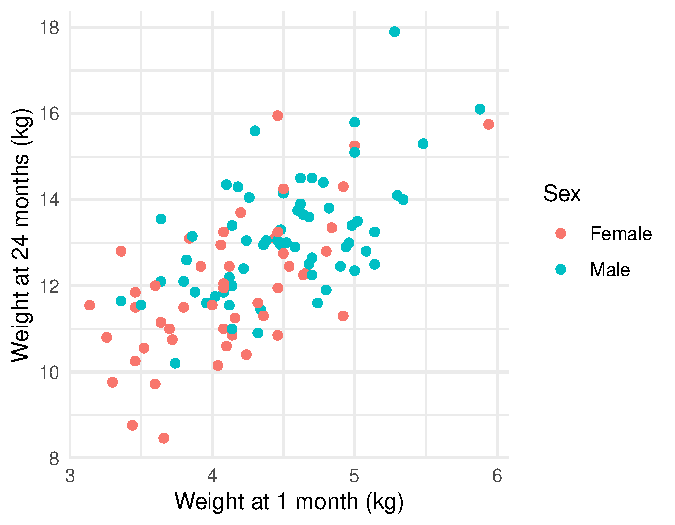
\includegraphics{Group-1-Project_files/figure-pdf/fig-scat-wt24-wt1-1.pdf}

}

\caption{\label{fig-scat-wt24-wt1}Relationship between child weight at
24 months and weight at 1 month by sex}

\end{figure}%

Figure~\ref{fig-scat-wt24-wt1} shows the relationship between the
child's weight at 24 months against the child's weight at 1 month. From
Figure~\ref{fig-scat-wt24-wt1} it appears that there is a positive,
moderate to strong linear relationship between a child's weight at 24
months and weight at 1 month. Moreover, with the exception of a few
points there appears to be a distinction by gender with female children
having lower weight and male children having a higher weight.

\begin{table}

\begin{minipage}{0.50\linewidth}

\begin{longtable*}{lrrr}
\toprule
term & Wt1 & Wt24 & Solids \\ 
\midrule\addlinespace[2.5pt]
Wt1 & $1.00$ & $0.56$ & $-0.13$ \\ 
Wt24 & $0.56$ & $1.00$ & $-0.07$ \\ 
Solids & $-0.13$ & $-0.07$ & $1.00$ \\ 
\bottomrule
\end{longtable*}

\end{minipage}%
%
\begin{minipage}{0.50\linewidth}

\begin{longtable*}{lrrr}
\toprule
term & Wt1 & Wt24 & Solids \\ 
\midrule\addlinespace[2.5pt]
Wt1 & $1.00$ & $0.64$ & $-0.23$ \\ 
Wt24 & $0.64$ & $1.00$ & $-0.37$ \\ 
Solids & $-0.23$ & $-0.37$ & $1.00$ \\ 
\bottomrule
\end{longtable*}

\end{minipage}%

\caption{\label{tbl-corrs}Correlations between numerical variables by
sex}

\end{table}%

Table~\ref{tbl-corrs} shows the correlation between numerical variables
for male and female children. From \textbf{?@tbl-corrs-1} we can see
that for males Wt1 and Wt24 are moderately, positivly correlated,
whereas Solids against Wt24 and Wt1 are weakly negatively correlated.
\textbf{?@tbl-corrs-2} highlights that this is slightly different for
female children as there appears to be a higher positive correlation
between Wt24 and Wt1. Additionally, there appears to be a moderate
negative correlation between Solids and Wt24 for female children and a
weak-moderate correlation between Solids and Wt1. This suggests that
there may be an interaction between Wt1 and Solids by Sex.

\begin{longtable}{lrrrrrrrrr}

\caption{\label{tbl-summary}Mean, median and standard deviation (sd)
Wt24, Wt1 and Solids by sex.}

\tabularnewline

\toprule
 & \multicolumn{3}{c}{Wt24} & \multicolumn{3}{c}{Wt1} & \multicolumn{3}{c}{Solids} \\ 
\cmidrule(lr){2-4} \cmidrule(lr){5-7} \cmidrule(lr){8-10}
Sex & Mean & Median & Std.Dev & Mean & Median & Std.Dev & Mean & Median & Std.Dev \\ 
\midrule\addlinespace[2.5pt]
Male & $13.12$ & $13.03$ & $1.35$ & $4.51$ & $4.51$ & $0.52$ & $11.50$ & $11.00$ & $3.18$ \\ 
Female & $11.94$ & $11.85$ & $1.59$ & $4.11$ & $4.08$ & $0.55$ & $11.43$ & $12.00$ & $2.91$ \\ 
\bottomrule

\end{longtable}

Table~\ref{tbl-summary} shows the mean, median and standard deviation of
Wt24, Wt1 and Solids by Sex. Table~\ref{tbl-summary} highlights that
there appears to be a slight difference between Wt24 by sex.
Additionally, There does not appear to be a difference in Wt1 and Solids
by sex.

\begin{figure}

\centering{

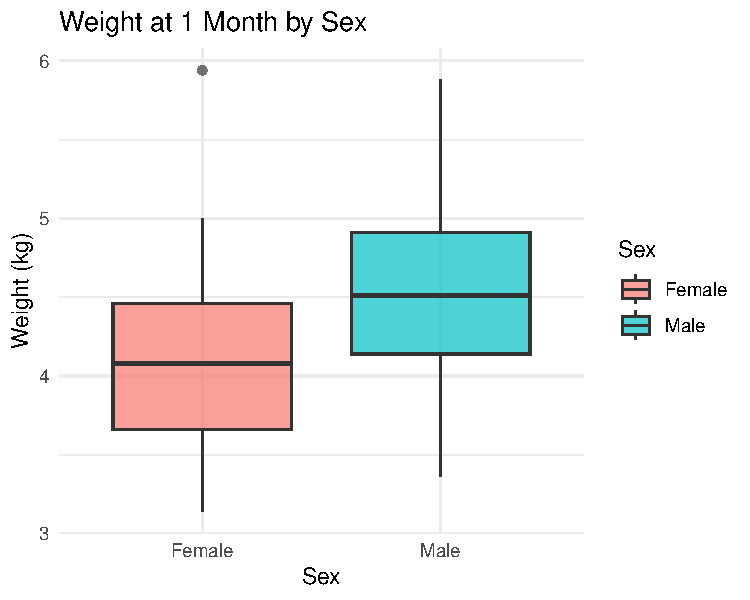
\includegraphics{Group-1-Project_files/figure-pdf/fig-box-wt1-1.pdf}

}

\caption{\label{fig-box-wt1}Distribution of weight at 1 month by sex}

\end{figure}%

Figure~\ref{fig-box-wt1} presents a boxplot illustrating the
distribution of weight at 1 month categorized by sex. The plot suggests
that male infants tend to have a slightly higher median weight compared
to females, with a slightly wider range of values. The presence of
outliers, particularly among female infants, indicates some variation in
early weight distribution.

\begin{figure}

\centering{

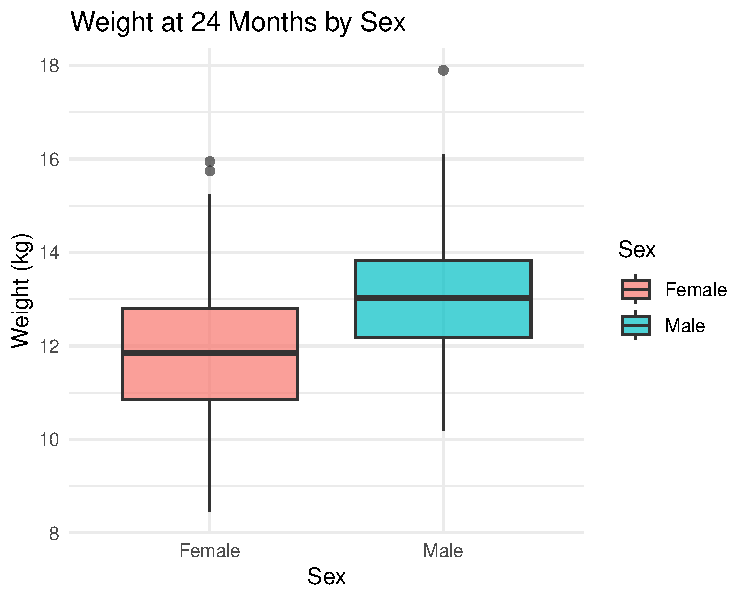
\includegraphics{Group-1-Project_files/figure-pdf/fig-box-wt24-1.pdf}

}

\caption{\label{fig-box-wt24}Distribution of weight at 24 months by sex}

\end{figure}%

Figure~\ref{fig-box-wt24} extends this analysis to weight at 24 months,
where the observed trend continues. Male children exhibit a higher
median weight than female children, and the overall distribution of
weight is more spread out for males. The increased variation,
particularly in the upper range, suggests that male children may
experience a broader range of growth trajectories compared to females.

\begin{figure}

\centering{

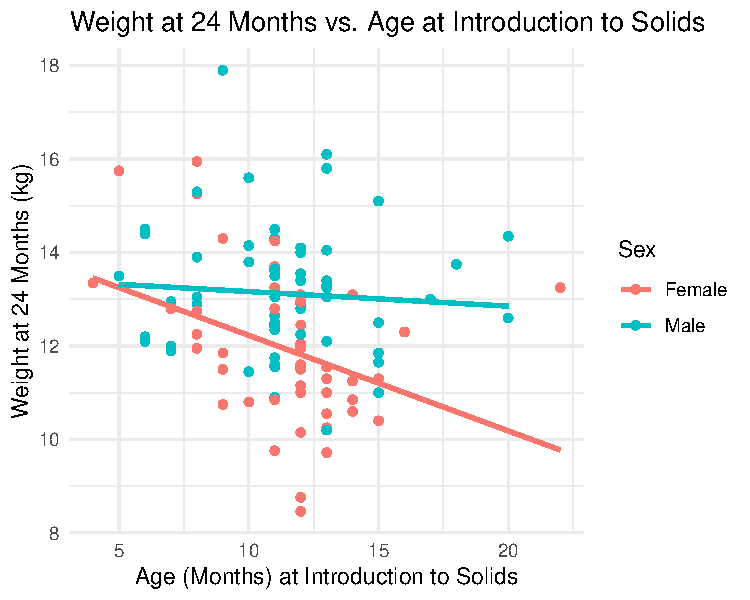
\includegraphics{Group-1-Project_files/figure-pdf/fig-scat-wt24-solids-1.pdf}

}

\caption{\label{fig-scat-wt24-solids}Relationship between weight at 24
months and age at introduction to solids, colored by sex}

\end{figure}%

Figure~\ref{fig-scat-wt24-solids} illustrates the relationship between
weight at 24 months (Wt24) and the age at which solid foods were
introduced (Solids), with separate regression lines for males and
females. The plot suggests a slight negative trend for females,
indicating that introducing solids later may be associated with lower
weight at 24 months. In contrast, the regression line for males remains
relatively flat, suggesting a weaker or negligible relationship between
solid food introduction and weight at 24 months for male children.

\subsection{References}\label{references}

\url{https://www.nhs.uk/conditions/baby/babys-development/height-weight-and-reviews/baby-height-and-weight/}

\url{https://www.babycenter.com/baby/baby-development/average-weight-and-growth-chart-for-babies-toddlers-and-beyo_10357633}



\end{document}
